\section{Plateforme similaire à notre étude}

\subsubsection{freeStep de Sensor Medica}
Cette solution logicielle complète permet l'évaluation de la distribution plantaire, l'analyse biomécanique du mouvement des membres inférieurs et l'étude de la posture corporelle. 
Elle intègre divers dispositifs pour des analyses biomécaniques et thermiques approfondies.

\begin{figure}[ht]
    \centering
    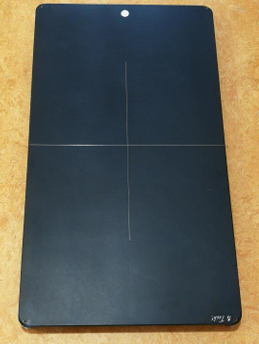
\includegraphics[width=0.5\textwidth]{images/freestep.png}
    \caption{Interface de freeStep}
    \label{fig:freestep}
\end{figure}